\documentclass[tikz]{standalone}

\begin{document}
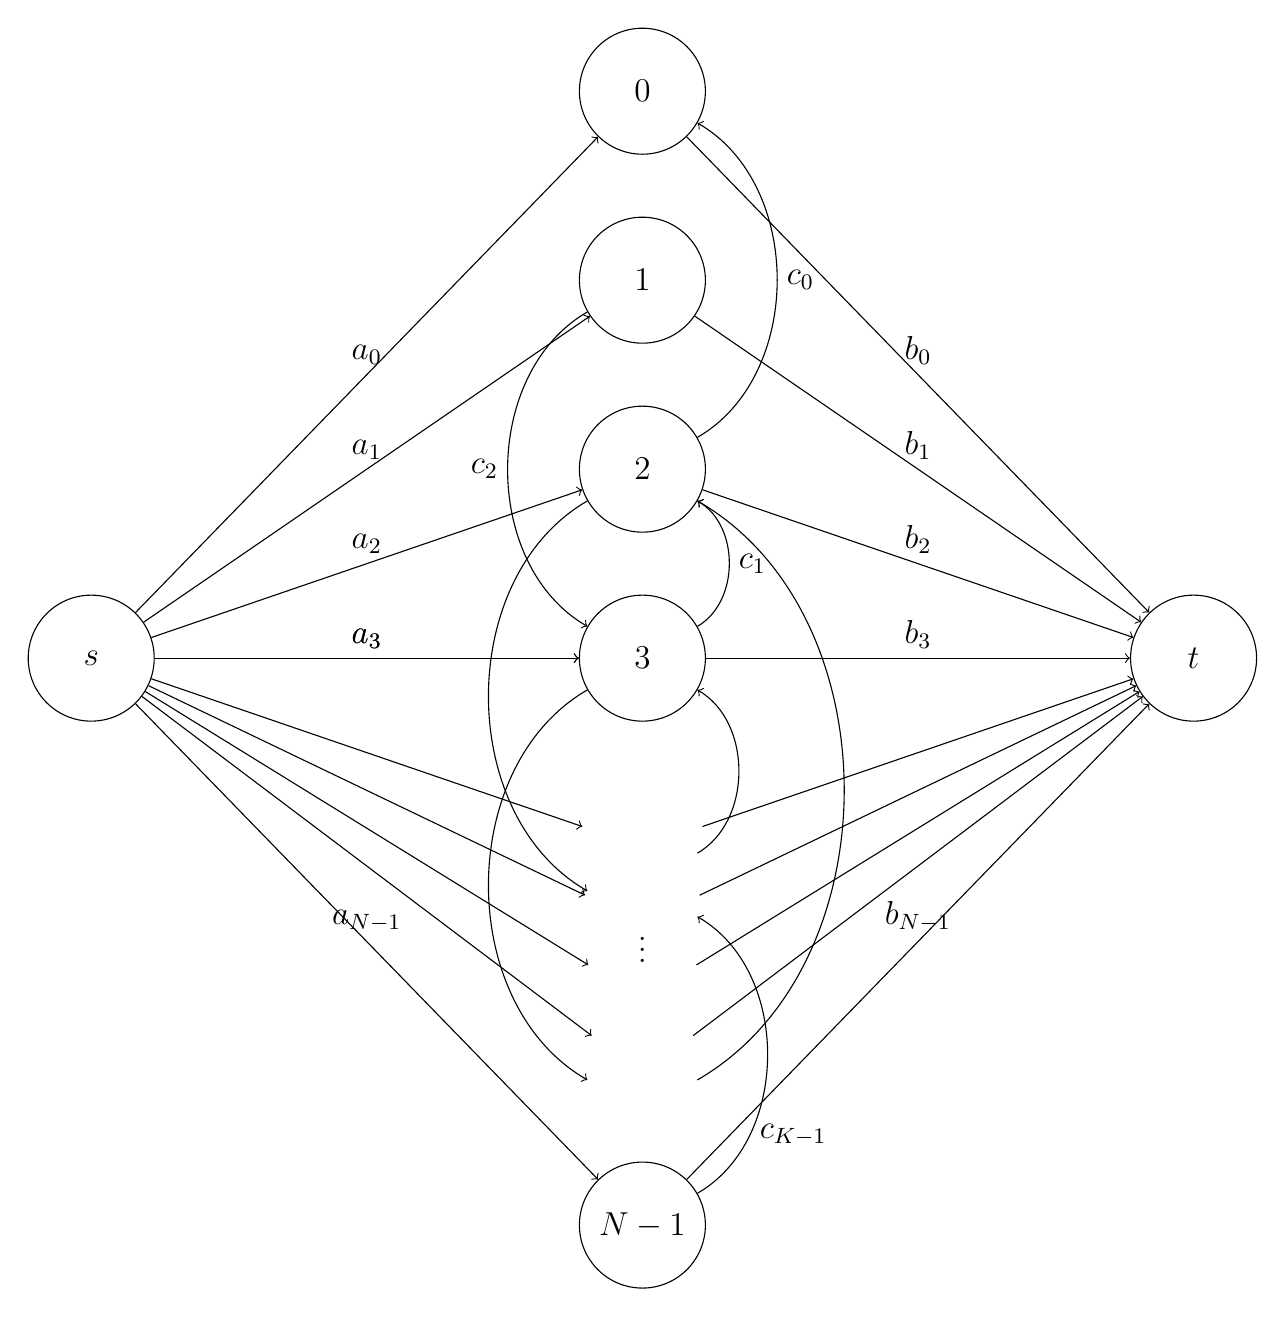
\begin{tikzpicture}[
    x=7.0cm,
    y=2.4cm,
    font=\large,
    v/.style={draw, circle, fill=white, minimum size=1.6cm},
    dots/.style={circle, minimum size=1.6cm},
    e/.style={draw, ->},
]
    \node[v] (s) at (-1, 0) {$s$};
    \node[v] (x0) at (0, 3) {$0$};
    \node[v] (x1) at (0, 2) {$1$};
    \node[v] (x2) at (0, 1) {$2$};
    \node[v] (x3) at (0, 0) {$3$};
    \node at (0, -1.5) {$\vdots$};
    \node[dots] (dots0) at (0, -1.0) {};
    \node[dots] (dots1) at (0, -1.2) {};
    \node[dots] (dots2) at (0, -1.4) {};
    \node[dots] (dots3) at (0, -1.6) {};
    \node[dots] (dots4) at (0, -1.8) {};
    \node[dots] (dots5) at (0, -2.0) {};
    \node[dots] (dots6) at (0, -2.2) {};
    \node[dots] (dots7) at (0, -2.4) {};
    \node[v] (xl) at (0, -3) {$N-1$};
    \node[v] (t) at (1, 0) {$t$};

    \path[e] (s) edge node[midway, above] {$a_0$} (x0);
    \path[e] (s) edge node[midway, above] {$a_1$} (x1);
    \path[e] (s) edge node[midway, above] {$a_2$} (x2);
    \path[e] (s) edge node[midway, above] {$a_3$} (x3);
    \path[e] (s) edge node[midway, above] {$a_3$} (x3);
    \path[e] (s) edge (dots0);
    \path[e] (s) edge (dots2);
    \path[e] (s) edge (dots4);
    \path[e] (s) edge (dots6);
    \path[e] (s) edge node[midway, above] {$a_{N-1}$} (xl);
    \path[e] (x0) edge node[midway, above] {$b_0$} (t);
    \path[e] (x1) edge node[midway, above] {$b_1$} (t);
    \path[e] (x2) edge node[midway, above] {$b_2$} (t);
    \path[e] (x3) edge node[midway, above] {$b_3$} (t);
    \path[e] (dots0) edge (t);
    \path[e] (dots2) edge (t);
    \path[e] (dots4) edge (t);
    \path[e] (dots6) edge (t);
    \path[e] (xl) edge node[midway, above] {$b_{N-1}$} (t);

    \path[e, out=30, in=-30] (x2) edge node[midway, right] {$c_0$} (x0);
    \path[e, out=30, in=-30] (x3) edge node[midway, right] {$c_1$} (x2);
    \path[e, out=-150, in=150] (x1) edge node[midway, left] {$c_2$} (x3);
    \path[e, out=30, in=-30] (dots1) edge (x3);
    \path[e, out=30, in=-30] (dots7) edge (x2);
    \path[e, out=30, in=-30] (xl) edge node[near start, right] {$c_{K-1}$} (dots1);
    \path[e, out=-150, in=150] (x2) edge (dots2);
    \path[e, out=-150, in=150] (x3) edge (dots7);
\end{tikzpicture}
\end{document}
